\documentclass{standalone}
\usepackage[dvipsnames,svgnames,x11names]{xcolor}
\usepackage{tikz}
\usepackage{pgfplots}
\usetikzlibrary{pgfplots.statistics}
\pgfplotsset{compat = 1.12}
\usepackage[
  group-separator={,},
  exponent-product=\cdot,
]{siunitx}
\usepackage{../thesismath}
\begin{document}
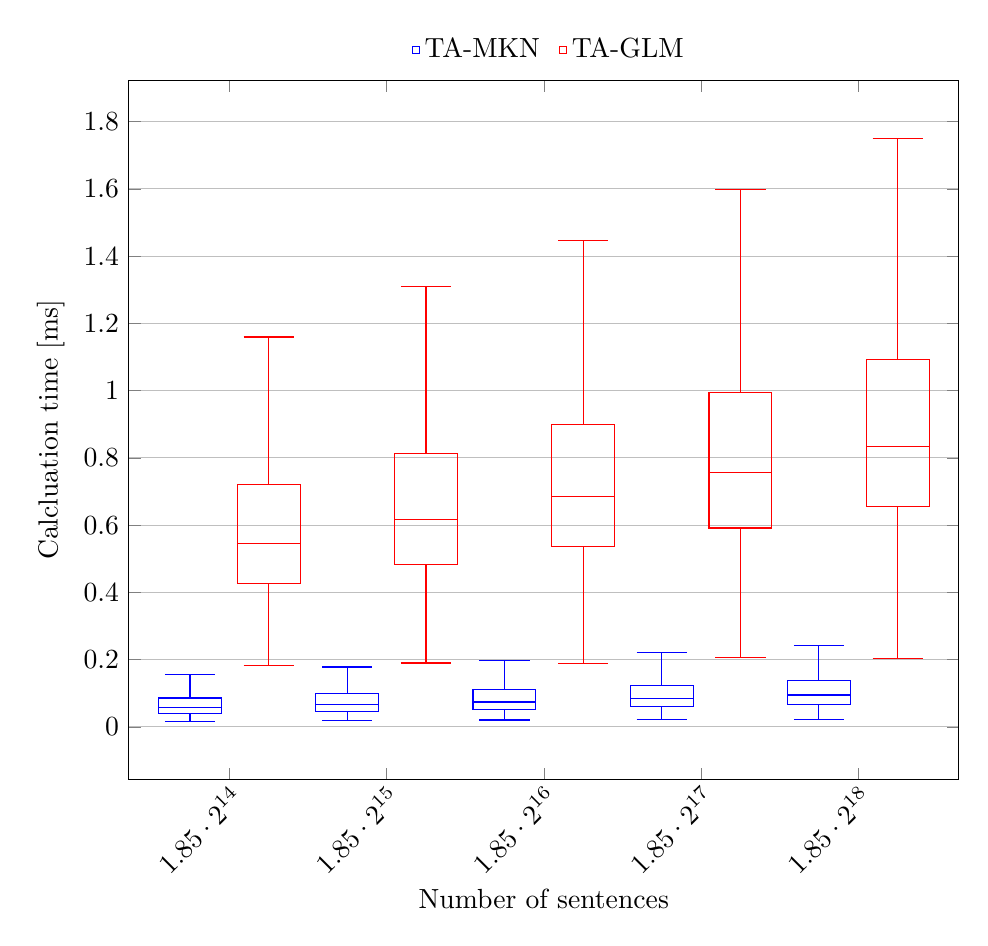
\begin{tikzpicture}[baseline]

\pgfplotscreateplotcyclelist{mkn_glm}{%
  blue,  mark size=1.25, mark=square,\\%
  red,   mark size=1.25, mark=square,\\%
}

\pgfplotsset{
  legend style = {
    draw = none,
    legend image code/.code = {
      \draw[only marks]
        plot coordinates {
          (0.3cm,0cm)
        };
      \node at (0.15cm, 0cm) {};
    },
  },
  boxplot/draw/average/.code = {
    %% uncomment to show dotted bars for average:
    %\draw[dashed, /pgfplots/boxplot/every average/.try]
    %  (boxplot box cs:\pgfplotsboxplotvalue{average},0)
    %  --
    %  (boxplot box cs:\pgfplotsboxplotvalue{average},1)
    %  ;
  },
}

\sisetup{exponent-base = 2}
\begin{axis}[
  xlabel = {Number of sentences},
  xtick       = {            1,             2,             3,             4,             5},
  xticklabels = {\num{1.85e14}, \num{1.85e15}, \num{1.85e16}, \num{1.85e17}, \num{1.85e18}},
  xticklabel style={
    inner sep = 1pt,
    anchor = north east,
    rotate = 45,
  },
  ylabel = {Calcluation time [\si{\milli\second}]},
  scaled y ticks = false,
  log ticks with fixed point,
  boxplot/draw direction = y,
  cycle list name = mkn_glm,
  grid = major,
  xmajorgrids = false,
  legend entries = {{TA-MKN}, {TA-GLM}},
  legend style = {
    anchor=south,
    at={(axis description cs: 0.5, 1.01)}
  },
  legend columns = 3,
  width = \textwidth,
]

% training-5-argmaxcompare-40k-c/ngram-5-TA-Weighted-Sum-Modified-Kneser-Ney-1
\addplot+[
  boxplot prepared = {
    %draw position = 30400,
    draw position = 1,
    box extend = 0.4,
    lower whisker = 0.017048,
    lower quartile = 0.039706,
    median = 0.058548,
    upper quartile = 0.085849,
    upper whisker = 0.155036,
    average = 0.071223,
  },
  xshift = -0.5cm,
] table [row sep = \\, y index = 0] {
  data\\
};

% training-5-argmaxcompare-40k-c/ngram-5-TA-Weighted-Sum-Generalized-Language-Model-1
\addplot+[
  boxplot prepared = {
    %draw position = 30400,
    draw position = 1,
    box extend = 0.4,
    lower whisker = 0.182297,
    lower quartile = 0.427452,
    median = 0.545453,
    upper quartile = 0.720338,
    upper whisker = 1.159506,
    average = 0.614068,
  },
  xshift = 0.5cm,
] table [row sep = \\, y index = 0] {
  data\\
};

% ------------------------------------------------------------------------------

% training-4-argmaxcompare-40k-c/ngram-5-TA-Weighted-Sum-Modified-Kneser-Ney-1
\addplot+[
  boxplot prepared = {
    %draw position = 60801,
    draw position = 2,
    box extend = 0.4,
    lower whisker = 0.019755,
    lower quartile = 0.045715,
    median = 0.066753,
    upper quartile = 0.098698,
    upper whisker = 0.178131,
    average = 0.081448,
  },
  xshift = -0.5cm,
] table [row sep = \\, y index = 0] {
  data\\
};

% training-4-argmaxcompare-40k-c/ngram-5-TA-Weighted-Sum-Generalized-Language-Model-1
\addplot+[
  boxplot prepared = {
    %draw position = 60801,
    draw position = 2,
    box extend = 0.4,
    lower whisker = 0.189782,
    lower quartile = 0.483218,
    median = 0.617765,
    upper quartile = 0.813524,
    upper whisker = 1.308804,
    average = 0.692814,
  },
  xshift = 0.5cm,
] table [row sep = \\, y index = 0] {
  data\\
};


% ------------------------------------------------------------------------------

% training-3-argmaxcompare-40k-c/ngram-5-TA-Weighted-Sum-Modified-Kneser-Ney-1
\addplot+[
  boxplot prepared = {
    %draw position = 121602,
    draw position = 3,
    box extend = 0.4,
    lower whisker = 0.020270,
    lower quartile = 0.051889,
    median = 0.074050,
    upper quartile = 0.110448,
    upper whisker = 0.198268,
    average = 0.090352,
  },
  xshift = -0.5cm,
] table [row sep = \\, y index = 0] {
  data\\
};

% training-3-argmaxcompare-40k-c/ngram-5-TA-Weighted-Sum-Generalized-Language-Model-1
\addplot+[
  boxplot prepared = {
    %draw position = 121602,
    draw position = 3,
    box extend = 0.4,
    lower whisker = 0.187163,
    lower quartile = 0.535744,
    median = 0.685056,
    upper quartile = 0.899978,
    upper whisker = 1.446284,
    average = 0.771727,
  },
  xshift = 0.5cm,
] table [row sep = \\, y index = 0] {
  data\\
};

% ------------------------------------------------------------------------------

% training-2-argmaxcompare-40k-c/ngram-5-TA-Weighted-Sum-Modified-Kneser-Ney-1
\addplot+[
  boxplot prepared = {
    %draw position = 2432004,
    draw position = 4,
    box extend = 0.4,
    lower whisker = 0.021501,
    lower quartile = 0.059342,
    median = 0.084170,
    upper quartile = 0.124255,
    upper whisker = 0.221622,
    average = 0.101046,
  },
  xshift = -0.5cm,
] table [row sep = \\, y index = 0] {
  data\\
};

% training-2-argmaxcompare-40k-c/ngram-5-TA-Weighted-Sum-Generalized-Language-Model-1
\addplot+[
  boxplot prepared = {
    %draw position = 2432004,
    draw position = 4,
    box extend = 0.4,
    lower whisker = 0.207189,
    lower quartile = 0.591446,
    median = 0.755523,
    upper quartile = 0.994264,
    upper whisker = 1.598150,
    average = 0.855940,
  },
  xshift = 0.5cm,
] table [row sep = \\, y index = 0] {
  data\\
};

% ------------------------------------------------------------------------------

% training-1-argmaxcompare-40k-c/ngram-5-TA-Weighted-Sum-Modified-Kneser-Ney-1
\addplot+[
  boxplot prepared = {
    %draw position = 486409,
    draw position = 5,
    box extend = 0.4,
    lower whisker = 0.022592,
    lower quartile = 0.066967,
    median = 0.094754,
    upper quartile = 0.136932,
    upper whisker = 0.241880,
    average = 0.111001,
  },
  xshift = -0.5cm,
] table [row sep = \\, y index = 0] {
  data\\
};

% training-1-argmaxcompare-40k-c/ngram-5-TA-Weighted-Sum-Generalized-Language-Model-1
\addplot+[
  boxplot prepared = {
    %draw position = 486409,
    draw position = 5,
    box extend = 0.4,
    lower whisker = 0.202749,
    lower quartile = 0.654436,
    median = 0.832421,
    upper quartile = 1.092418,
    upper whisker = 1.749261,
    average = 0.952469,
  },
  xshift = 0.5cm,
] table [row sep = \\, y index = 0] {
  data\\
};

\end{axis}

\end{tikzpicture}
\end{document}
